\documentclass[12pt,letterpaper]{article}
\usepackage[margin=1.5in]{geometry}
\usepackage[english]{babel}
\usepackage[utf8x]{inputenc}
\usepackage{amsmath}
\usepackage{amssymb} 
\usepackage[retainorgcmds]{IEEEtrantools}
\usepackage{graphicx}
\usepackage{tabularx}
\usepackage{subfig}
\usepackage{kpfonts}    % for nice fonts
\usepackage{microtype} 
\usepackage{booktabs}   % for nice tables
\usepackage{bm}         % for bold math
\usepackage{listings}   % for inserting code
\usepackage{verbatim}   % useful for program listings
\usepackage{color}  
\usepackage[colorlinks=true]{hyperref}
% use for hypertext
\usepackage[colorinlistoftodos]{todonotes}
\usepackage{natbib}

\hypersetup{
    colorlinks=true,
    linkcolor=blue, 
    filecolor=magenta, 
    urlcolor=cyan,
    citecolor=magenta 
}

\begin{document}

\section{Model \& Assumptions}

We assume there are two \textit{symmetric} firms indexed by $i\in\{1,-1\}$ competing on prices given a finite discrete horizon $t=\{T,T-1,\cdots,1,0\}$. At each time $t$, each firm $i$ can set price $p_{it}\in\{p_l,p_h\}$\footnote{This simplification borrows from \cite{miklos2019collusion}.}, where $0<p_l<p_h$. The price vector is denoted by $p_t$. 

Each period, there is a potential customer with probability $\lambda<1$, and we assume the demand follows the logit function:

\[
    q_i(p_t) = \frac{\exp(a-bp_i)}{1+\sum_{i\in\{1,-1\}}\exp(a-bp_i) }
\]

where $a, b$ should satisfy $a>0, b>0, a-bp_h\ge0$.

For simplicity, we could write the purchasing probability as:

\[
    q_{ll} = \frac{\exp(a-bp_l)}{1+2\exp(a-bp_l)}, q_{lh} = \frac{\exp(a-bp_l)}{1+\exp(a-bp_l)+\exp(a-bp_h)};
\]

\[
    q_{hl} = \frac{\exp(a-bp_h)}{1+\exp(a-bp_l)+\exp(a-bp_h)}, q_{hh} = \frac{\exp(a-bp_h)}{1+2\exp(a-bp_h)}.
\]

i.e. $q_{xy}$ denotes the demand function for firm $i$ when the price vector $(p_i,p_{-i})$ is $p_x,p_y$. 

At time $T$, each firm has a public initial capacity $s\ge0$. 

\section{Capacity as Public Information}

Assume that there is only one equilibrium and denote $V_i(s_i, s_{-i}, t)$ as the value function given the current state $(s_i, s_{-i}, t)$ when both firms price at the unique equilibrium. When one customer arrives at time $t$ and firm $i,-i$ set their prices at $p_x, p_y$ respectively, the revenue pair $\pi(p_x,p_y, ,s_i,s_{-i},t) = (\pi_i(p_x,p_y,s_i,s_{-i},t), \pi_{-i}(p_x,p_y,s_i,s_{-i},t))$ is given by:

\begin{align}
    \pi_i(p_x,p_y,s_i,s_{-i},t) &= q_{xy}\cdot (p_x+V_i(s_i-1,s_{-i},t-1)) + q_{yx}\cdot V_i(s_i, s_{-i}-1, t-1) \nonumber \\
    &\quad + (1-q_{xy}-q_{yx}) \cdot V_i(s_i,s_{-i},t-1) \nonumber \\
    \pi_{-i}(p_x,p_y,s_i,s_{-i},t) &= q_{xy}\cdot V_i(s_{-i}, s_i-1, t-1) + q_{yx}\cdot (p_y+V_i(s_{-i}-1, s_i, t-1)) \nonumber \\
    &\quad + (1-q_{xy}-q_{yx}) \cdot V_i(s_{-i},s_{i},t-1) \label{eq:revenue_pair}
\end{align}
    
Under the equilibrium price $p_x^*(s_i,s_{-i},t),p_y^*(s_i,s_{-i},t)$, the value function can be expressed by:

\begin{equation}\label{eq:value_function}
    V_i(s_i,s_{-i},t) =& \lambda \pi_i(p_x^*,p_y^*,s_i,s_{-i},t) + (1-\lambda) V_i(s_i,s_{-i},t-1) 
\end{equation}

The boundary condition is defined as:

\[
    V_i(0,s_{-i},t) = 0, v_i(s_i,s_{-i},0) = 0
\]

\textbf{Computation:} There are two components to calculate:

\begin{enumerate}
    \item The value function $V_i(s_i,s_{-i},t)$;
    \item The price pairs under equilibrium $p^*(s_i, s_{-i}, t)$.
\end{enumerate}

Given value function $V_i(\cdot, \cdot, t-1)$ known, $p^*(s_i, s_{-i}, t)$ can be computed by solving a tabular game. Given $V_i(\cdot, \cdot, t-1)$ and $p^*(s_i, s_{-i}, t)$ known, $V_i(\cdot, \cdot, t)$ can be computed directly. The detailed computation steps are given below:

\begin{enumerate}
    \item Write a function to return $q_{xy}$ given $a, b, p_h, p_l$ (examine parameters);
    \item Store $V_i(s_i,s_{-i},t)$ in a $s+1\times s+1\times T+1$-dimensional Numpy ndarray, and $P^*(s_i, s_{-i}, t)$ in a $s+1\times s+1\times T+1 \times 2$-dimensional Numpy ndarray, where the 2-dimensional tuple $P[s_{i}][s_{-i}][t]$ denotes the probability of choosing $p_h$ under the mixed-strategy equilibrium given the current state;
    \item Starting from the boundary condition, set $V_i(s_i, s_{-i}, 0)=0$ for all $(s_i, s_{-i})$, and set $V_i(0, s_{-i}, t)=0$ for all $(s_{-i}, t)$;
    \item To calculate $V_i(s_i,0,t)$, we need another dynamic programming. Consider the monopoly market where only firm $i$ sells its product and prices. We have:
    
    \[
        q_{l} = \frac{\exp(a-bp_l)}{1+\exp(a-bp_l)}, q_{h} = \frac{\exp(a-bp_h)}{1+\exp(a-bp_h)}
    \]

    Similar to the previous deduction:
    
    \[  
        \pi_i(p_x,s_i,t) = q_x \times  (p_x+\tilde{V}_i(s_i-1,t-1)) + (1-q_x) \times \tilde{V}_i(s_i,t-1)
    \]
    
    \[
        \begin{align}
            \tilde{V}_i(s_i,t) &= \lambda \pi_i(p^*,s_i,t) + (1-\lambda) \tilde{V}_i(s_i,t-1) \\
            &= \max_{p\in\{p_h,p_l\}} \lambda q_p (p+\tilde{V}_i(s_i-1,t-1)) + (1-\lambda q_p) \tilde{V}_i(s_i,t-1)
        \end{align}
        
    \]

    With boundary condition $\tilde{V}_i(0,t)=0, \tilde{V}_i(s_i,0)=0$, we can use backward iteration to solve all $\tilde{V}_i(s_i,t)$, and $\tilde{V}_i(s_i,t)= V_i(s_i,0,t)$.
    \item Set $t=1$, backwardly iterate the following steps until $t=T+1$:
    
    \begin{enumerate}
        \item Write the payoff matrix at time $t$ for all $(s_i,s_{-i})$:
        
        \begin{table}[h]
            \centering
            \begin{tabular}{|c|c|c|}
                \hline
                \textbf{Firm $i$} / \textbf{Firm $-i$} & $p_h$ & $p_l$ \\
                \hline
                $p_h$ & $\pi_i(p_h,p_h), \pi_{-i}(p_h,p_h)$ & $\pi_i(p_h,p_l), \pi_{-i}(p_h,p_l)$ \\
                \hline
                $p_l$ & $\pi_i(p_l,p_h), \pi_{-i}(p_l, p_h)$ & $\pi_i(p_l,p_l), \pi_{-i}(p_l,p_l)$ \\
                \hline
            \end{tabular}
            \caption{Payoff Matrix given $s_i,s_{-i}, t$}
            \label{tab:payoff1}
        \end{table}
        
        where the payoff is defined by Equations \ref{eq:revenue_pair};
        \item First, check if there is any pure-strategy NE. If not, solving the mixed-strategy equilibrium $p^*, q^*$ for all $(s_i, s_{-i})$, the solution has the closed-form form:

        \[
            p^* = \frac{\pi_{-i}(p_l,p_l)-\pi_{-i}(p_l,p_h)}{\pi_{-i}(p_h,p_h)-\pi_{-i}(p_h,p_l)+\pi_{-i}(p_l,p_l)-\pi_{-i}(p_l,p_h)}
        \]
        
        \[
            q^* = \frac{\pi_{i}(p_l,p_l)-\pi_{i}(p_h,p_l)}{\pi_{i}(p_h,p_h)-\pi_{i}(p_l,p_h)+\pi_{i}(p_l,p_l)-\pi_{i}(p_h,p_l)}
        \]
        
        where $p^*$ and $q^*$ are the probabilities selecting $p_h$ for firm $i$ and $-i$ under the equilibrium.
        \item Compute $V_i(s_i, s_{-i}, t+1)$ for all $(s_i, s_{-i})$ using Equation \ref{eq:value_function}. Due to the mixed-strategy equilibrium, the expression should be:

        \[
            \begin{align}
                V_i(s_i,s_{-i},t) & = (1-\lambda)V_i(s_i,s_{-i},t-1) \\
                & + \lambda \codt \{pq \pi_i(p_h,p_h,s_i,s_{-i},t) + (1-p)q \pi_i(p_l,p_h,s_i,s_{-i},t) \\
                & + p(1-q) \pi_i(p_h,p_l,s_i,s_{-i},t) + (1-p)(1-q) \pi_i(p_l,p_l,s_i,s_{-i},t) \}
            \end{align}
        \]
        \item $t+=1$.
    \end{enumerate}
\end{enumerate}

\textbf{Results:}

\begin{itemize}
    \item For all $s_i,s_{-i},t$, the equilibriums for game \ref{tab:payoff1} are pure-strategy equilibrium;
    \item The results are sensitive to the hyperparameters. When $b$ is small and the gap between $p_h,p_l$ is huge, all equilibriums would be $p_h, p_h$.
\end{itemize}

\section{Capacity as Private Information}

The initial capacity $s$ is public information; after that, each firm's demand remains private. Following the ideas in \cite{loots2023data}, we can infer the opponent's demand conditioning on one's own demand under the logit model. 

Specifically, when each firm observes its own demand of $1$, it knows the opponent's demand is $0$; when each firm observes its own demand of $0$, it updates the opponent's capacity using the Bayesian formula: $s'_{-i}-\frac{\lambda p_{yx}}{1-\lambda p_{xy}}$. Denote $V_i(s_i,s_{-i}',t)$ as the value function under the \textit{equilibrium strategy} when both firms assume that they have accurately estimated the opponent's capacity.\footnote{\textbf{Note} that the equilibrium strategy here means that when firm $i$ has the state $(s_i,s_{-i}',t)$, it will act as if it is in the public capacity setting and when the opponent has real capacity $s_{-i}^'$. This is a very strong assumption and is also used in the report in Cardinal Operations, and this assumption could lead to some problems in the computation process.}

We further assume each firm won't infer the opponent's demand from the opponent's historical prices. For example, when the firm's estimated opponent's capacity mismatches with the opponent's real capacity, the opponent's equilibrium price solved given $(s_i,s_{-i}',t)$ can misalign with the opponent's real action, then the firm would know $s_{-i}'$ is biased but wouldn't correct the estimated $s_{-i}'$. Under these assumptions, we have:

\[
    V_i(s_i,s_{-i}', t) = \lambda q_{x^*y^*}\cdot(p_{x^*}+V_i(s_i-1,s_{-i}',t-1)) + (1-\lambda q_{x^*y^*})\cdot V_i(s_i, s_{-i}'-\frac{\lambda q_{y^*x^*}}{1-\lambda q_{x^*y^*}}, t-1)
\]

However, this would make the state space continuous and the model untractable. We further make the following assumptions on the Bayesian updation in a stochastic manner: when one firm has a demand of $0$, it will update the state to $(s_i,s_{-i}^\prime-1,t-1)$ with probability $\frac{\lambda q_{y^*x^*}}{1-\lambda q_{x^*y^*}}$, or update to $(s_i,s_{-i}^\prime,t-1)$ with probability $\frac{1-\lambda q_{x^*y^*}-\lambda q_{y^*x^*}}{1-\lambda q_{x^*y^*}}$, thus we have:

\[
    \begin{align}
        V_i(s_i,s_{-i}', t) = & \lambda q_{x^*y^*}\cdot(p_{x^*}+V_i(s_i-1,s_{-i}',t-1)) + (1-\lambda q_{x^*y^*}) \\
        \cdot & \{ \frac{\lambda q_{y^*x^*}}{1-\lambda q_{x^*y^*}} (s_i,s_{-i}^\prime-1,t-1) + \frac{1-\lambda q_{x^*y^*}-\lambda q_{y^*x^*}}{1-\lambda q_{x^*y^*}} V_i(s_i, s_{-i}', t-1)  \}
    \end{align}
\]

This equation, however, is exactly the same as Equation \ref{eq:value_function}. It's unable to compute because each firm can not anticipate the opponent's action $y^*$, so the value updation function is wrong. We could mitigate this by defining the Bellman equation under \textbf{a broader state space}. Instead of thinking of the value function for a single firm, we construct the state space for the whole environment while all firms act as assumed before\footnote{I'm not sure whether the report by Cardinal Operations takes a similar process, but if not, the calculated value function could be biased.}:

\begin{enumerate}
    \item Two firms have the same public initial capacity, and each maintains an estimation of the opponent's capacity from the beginning. In each epoch, each firm would update the estimation using the Bayesian formula conditioning on its own demand in a stochastic manner;
    \item At each period, each firm $i$ will choose the price as if it is in the public price setting. However, they can not anticipate the opponent's price since the estimated capacity could be wrong;
    \item We define the new value function $V(s_i,s_{-i},s'_i,s'_{-i},t)$, where $s_i,s_{-i}$ are real capacity while $s'_{-i}$ is the estimated capacity of firm $i$ on firm $-i$. This value function represents the expected payoff for both firms given the above assumption;
    \item For a given state $(s_i,s_{-i},s'_i,s'_{-i},t)$ and an action pairs $x, y$\footnote{From the numerical results in the previous section, all}, we have the following transitions on the state:
    \begin{itemize}
        \item With probability $\lambda q_{xy}$, firm $i$ obtain demand $1$, the system obtain reward $p_x$;
            \begin{itemize}
                \item with probability $\frac{\lambda q_{xy}}{1-\lambda q_{yx}}$, firm $-i$ assumes firm $i$ has demand $1$. The state is transitioned to $(s_i-1,s_{-i},s'_i-1,s'_{-i},t-1)$;
                \item with probability $\frac{1-\lambda q_{yx}-\lambda q_{xy}}{1-\lambda q_{yx}}$, the state is transitioned to $(s_i-1,s_{-i},s'_i,s'_{-i},t-1)$.
            \end{itemize}
        \item With probability $\lambda q_{yx}$, firm $-i$ obtain demand $1$, the system obtain reward $p_y$;
            \begin{itemize}
                \item with probability $\frac{\lambda q_{yx}}{1-\lambda q_{xy}}$, firm $i$ assumes firm $-i$ has demand $1$. The state is transitioned to $(s_i,s_{-i}-1,s'_i,s'_{-i}-1,t-1)$;
                \item with probability $\frac{1-\lambda q_{yx}-\lambda q_{xy}}{1-\lambda q_{xy}}$, the state is transitioned to $(s_i,s_{-i}-1,s'_i,s'_{-i},t-1)$.
            \end{itemize}
        \item With probability $1-\lambda q_{xy} - \lambda q_{yx} $, both firms obtain demand $0$, the system obtain reward $p_y$.
            \begin{itemize}
                \item with probability $\frac{\lambda q_{xy}}{1-\lambda q_{yx}} \cdot \frac{\lambda q_{yx}}{1-\lambda q_{xy}}$, firm $-i$ assumes firm $i$ has demand $1$, and firm $i$ assumes firm $-i$ has demand $1$. The state is transitioned to $(s_i,s_{-i},s'_i-1,s'_{-i}-1,t-1)$;
                \item with probability $\frac{\lambda q_{xy}}{1-\lambda q_{yx}} \cdot \frac{1-\lambda q_{yx}-\lambda q_{xy}}{1-\lambda q_{xy}}$, the state is transitioned to $(s_i,s_{-i},s'_i-1,s'_{-i},t-1)$;
                \item with probability $\frac{1-\lambda q_{yx}-\lambda q_{xy}}{1-\lambda q_{yx}} \cdot \frac{\lambda q_{yx}}{1-\lambda q_{xy}}$, the state is transitioned to $(s_i,s_{-i},s'_i,s'_{-i}-1,t-1)$;
                \item with probability $\frac{1-\lambda q_{yx}-\lambda q_{xy}}{1-\lambda q_{yx}} \cdot \frac{1-\lambda q_{yx}-\lambda q_{xy}}{1-\lambda q_{xy}}$, the state is transitioned to $(s_i,s_{-i},s'_i,s'_{-i},t-1)$.
            \end{itemize}
    \end{itemize}
    \item The boundary conditions are: $V(\cdot,\cdot,\cdot,\cdot,0)=0, V(0,0,\cdot,\cdot,t)=0$. Similar to the previous section, we can use backward iteration to compute the value function when one $s_i$ or $s_{-i}'$ equals $0$, the details are omitted here;
    \item Here we make another minor assumption: each firm can observe whether another firm's capacity reaches $0$. This assumption can make it much easier to compute the boundary condition: $V(s_i,0,s'_i,s'_{-i},t)=V_i(s_i,0,t)$ and $V(0,s_{-i},s'_i,s'_{-i},t)=V_i(s_{-i},0,t)$.
\end{enumerate}

The Bellman equation could be written as:

\begin{align*}
    V(s_i,s_{-i},s_{i}',s'_{-i},t) &= \lambda q_{xy} \times & \{p_x + \frac{\lambda q_{xy}}{1-\lambda q_{yx}} V(s_i-1,s_{-i},s'_i-1,s'_{-i},t-1) \\
    && + \frac{1-\lambda q_{yx}-\lambda q_{xy}}{1-\lambda q_{yx}} V(s_i-1,s_{-i},s'_i,s'_{-i},t-1) \} \\
    & + \lambda q_{yx} \times & \{p_y + \frac{\lambda q_{yx}}{1-\lambda q_{xy}} V(s_i,s_{-i}-1,s'_i,s'_{-i}-1,t-1) \\
    && + \frac{1-\lambda q_{yx}-\lambda q_{xy}}{1-\lambda q_{xy}} V(s_i,s_{-i}-1,s'_i,s'_{-i},t-1) \} \\
    & + (1-\lambda q_{xy} - \lambda q_{yx}) \times & \{ \frac{\lambda q_{xy}}{1-\lambda q_{yx}} \cdot \frac{\lambda q_{yx}}{1-\lambda q_{xy}} V(s_i,s_{-i},s'_i-1,s'_{-i}-1,t-1)  \\
    && +\frac{\lambda q_{xy}}{1-\lambda q_{yx}} \cdot \frac{1-\lambda q_{yx}-\lambda q_{xy}}{1-\lambda q_{xy}} \cdot V(s_i,s_{-i},s'_i-1,s'_{-i},t-1) \\
    && + \frac{1-\lambda q_{yx}-\lambda q_{xy}}{1-\lambda q_{yx}} \cdot \frac{\lambda q_{yx}}{1-\lambda q_{xy}} \cdot V(s_i,s_{-i},s'_i,s'_{-i}-1,t-1) \\
    && + \frac{1-\lambda q_{yx}-\lambda q_{xy}}{1-\lambda q_{yx}} \cdot \frac{1-\lambda q_{yx}-\lambda q_{xy}}{1-\lambda q_{xy}} \cdot V(s_i,s_{-i},s'_i,s'_{-i},t-1) \}
\end{align*}

\subsection{Other Explorations}

To handle the strong assumption that both firms will price based on the value function calculated under the public capacity setting, I also tried some other directions to mitigate this issue, but these directions all seem not working.

\begin{itemize}
    \item Consider a game where only one firm can observe both firms' capacity, but another firm only has its own capacity information. Similarly, the party who has the full information does not know the estimation of the limited-information one, so it can not predict the opponent's pricing, and the Bellman equation could not be written.
    \item Using Bayesian Nash Equilibrium (BNE) or Perfect Bayesian Equilibrium (PBE) to model the pricing behavior.
\end{itemize}

\section{Comparisons}

The parameter setting is given as: $\lambda = 0.2, a=5, b=0.2, p_h=12, p_l=10$. Figure \ref{fig:ratio1} and \ref{fig:ratio2} depict the ratio of the value function for the opaque setting to that of the transparent setting, across various demand-to-capacity ratios. The value function ratio is calculated by $\frac{V(s,s,s,s,T)/2}{V_i(s,s,T)}$, and the demand-to-capacity ratio is given by $\frac{\lambda \cdot T}{2s}$.

\begin{figure}
    \centering
    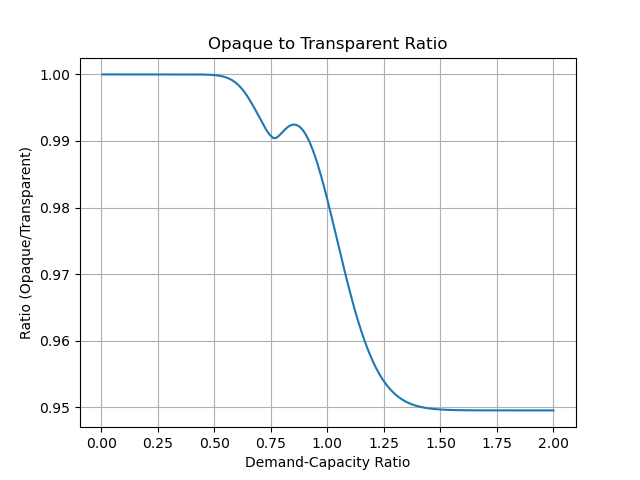
\includegraphics[width=0.5\linewidth]{pic/ratio1.png}
    \caption{$V(20,20,20,20,t)/2$ v.s. $V_i(20,20,t)$}
    \label{fig:ratio1}
\end{figure}


\begin{figure}
    \centering
    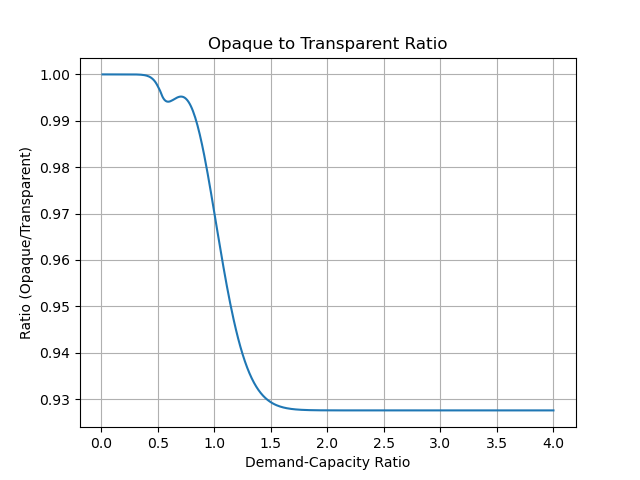
\includegraphics[width=0.5\linewidth]{pic/ratio2.png}
    \caption{$V(10,10,10,10,t)/2$ v.s. $V_i(10,10,t)$}
    \label{fig:ratio2}
\end{figure}

We can observe that both figures demonstrate an oblique `S' shape. But instead of the results in Cardinal Operations, which suggest that the value ratio will surpass $1$ when the demand-capacity ratio approaches $1$, it drops down quickly to a lower level.

\begin{figure}
    \centering
    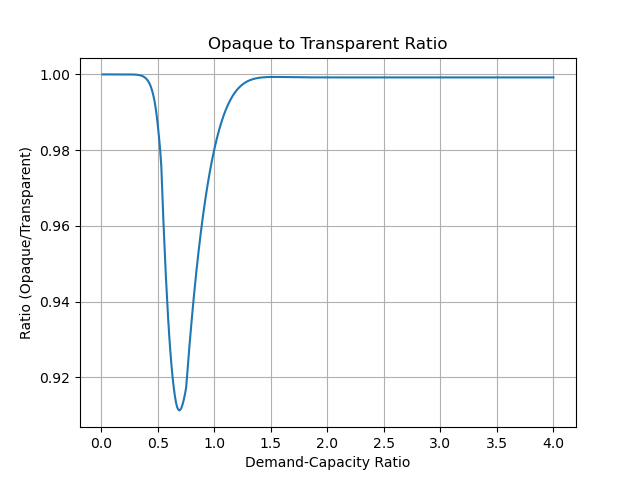
\includegraphics[width=0.5\linewidth]{pic/ratio3.png}
    \caption{$V(10,10,20,20,t)/2$ v.s. $V_i(10,10,t)$}
    \label{fig:ratio3}
\end{figure}

Figure \ref{fig:ratio3} indicates the case when both firms overestimate the initial capacity; we can see that the revenue ratio reapproaches $1$ when the demand-capacity ratio surpasses $1$.

\begin{figure}
    \centering
    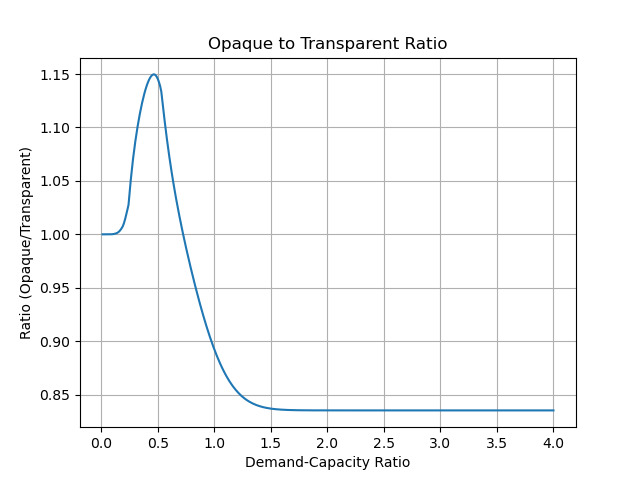
\includegraphics[width=0.5\linewidth]{pic/ratio4.png}
    \caption{$V(10,10,5,5,t)/2$ v.s. $V_i(10,10,t)$}
    \label{fig:ratio4}
\end{figure}

\begin{figure}
    \centering
    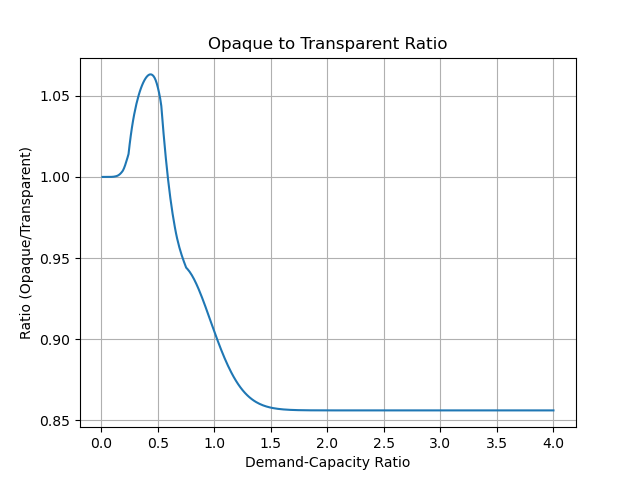
\includegraphics[width=0.5\linewidth]{pic/ratio5.png}
    \caption{$V(10,10,5,20,t)/2$ v.s. $V_i(10,10,t)$}
    \label{fig:ratio5}
\end{figure}

Figure \ref{fig:ratio4} indicates the case when both firms underestimate another firm's initial capacity, and figure \ref{fig:ratio5} indicates the case when one firm underestimates another firm's initial capacity while the other firm overestimates the opponent's capacity.

\bibliographystyle{apalike}
\bibliography{reference}
\end{document}